\documentclass[simplex.tex]{subfiles}
% NO NEED TO INPUT PREAMBLES HERE
% packages are inherited from simplex.tex; you can compile this on its own

\onlyinsubfile{
\title{NeuroData SIMPLEX Report: Subfile}
}

\begin{document}
\onlyinsubfile{
\maketitle
\thispagestyle{empty}

The following report documents the progress made by the labs of Randal~Burns and Joshua~T.~Vogelstein at Johns Hopkins University towards goals set by the DARPA SIMPLEX grant.

%%%% Table of Contents
\tableofcontents

%%%% Publications
\bibliographystyle{IEEEtran}
\begin{spacing}{0.5}
\section*{Publications, Presentations, and Talks}
\vspace{-20pt}
\nocite{*}
{\footnotesize	\bibliography{simplex}}
\end{spacing}
%%%% End Publications
}

\subsection{ndstore}

We have now added a resource RESTful service which allows users to create, list and delete project management information. This service is very useful for power users to manage their projects without having to log into the management console.


We continue to improve our caching layer in the cloud. We have now added a cache manager which manages the Redis cache for ndstore. The manager monitors the cache and starts evicting data when the data in cache exceeds a pre-set limit. This allows for efficient management of Redis memory and data can be moved transparently. We also implemented a Readers-Writer Lock using Redis atomic services. This lock can be now used by different processes using the redis-client. We plan to work towards trying to add this lock into the open-source redis-py client.


We continue to enable authentication for ndstore and converting all RESTful calls to HTTPS from HTTP. We have two different ways to authenticate to ndstore for different use-cases. First, a single persistent token for ndio users who should authenticate for every RESTful call. This token can be downloaded from the management console as a secret token and saved locally by the ndio user. Second, ephemeral session tokens for third-party applications which can authenticate users via a login screen. Third-party applications forward these credentials to the authentication server for session based tokens. The use case for this are applications are \itshape{ndviz, ndtilecache, CATMAID,} etc. This feature is under active development and is undergoing integration and testing. We also added continuous integration for automated testing with Travis--CI. This enables running our tests automatically for every commit. 


All existing data projects currently ingested indo ndstore have been migrated to the cloud. In addition, services for MRI data ingesting have been integrated and the BNU1 dataset has begun to be ingested into ndstore (Figure below), and a slice can be accessed at the following link: 
\href{http://mri.neurodata.io/nd/ca/BNU1/DTI_0025906_1/xy/0/0,182/0,218/90/1/}{http://mri.neurodata.io/nd/ca/BNU1/DTI\_0025906\_1/xy/0/0,182/0,218/90/1/}.  

\begin{figure}[h!]
\begin{cframed}
\centering
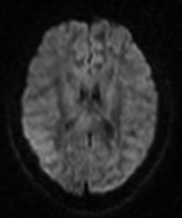
\includegraphics[width=2in]{../../figs/ndstore.png}
\caption{
A new tile interface was added to support filtered metadata tiles. Previously, when the user wanted to visualize an annotation project, all annotations were rendered as different colors based on ID. The filtered metadata tiles service allows the user to specify which annotation IDs to include when the tile is rendered. Using the service, combined with the RAMON Metadata services described in ndramondb below, a user can dynamically filter for specific IDs (e.g. all synapses), resulting in a cleaner and simpler view. 
}
\label{fig:ndstore}
\end{cframed}
\end{figure}


\subsubsection{ndingest}

Ingest is required to get data into our infrastructure.  Our existing ingest capabilities are limited by our hardware, which lacks in arbitrary scalability, both for a single user and multiple simultaneous users.  We therefore are building \textit{ndingest}, a submodule which supports interactions with the AWS cloud services specific to neurodata. This will be primarily used by the auto-ingest service to enable parallel ingest to AWS S3 buckets. The auto-ingest service has now been redesigned to use AWS lambda in conjunction with SQS, S3 and DynamoDB. 


We have now built wrappers for AWS lambda, SQS, S3 and DynamoDB  in \textit{ndingest}. The next stage is to write AWS security policies and ARN roles so that different aspects of these services can communicate with each other in the cloud. We are also developing scripts to deploy these services or update configurations from the command line. In addition, we have also developed a migration script to migrate our existing data to the cloud. This is essential since \textit{ndingest} is designed to ingest raw data not data already in ndstore.


We have also developed an ingest-client with JHU-APL to allow users to be able to use this service. The ingest-client is designed to be modular allowing users to add their respective plugins which match their data naming conventions. This is an improvement over the earlier phase where users had to convert their data to match a standard naming convention. This tool is also complemented with an ingest service which allows users to create, join, track and delete ingest jobs. 

\end{document}
